\subsection{Muons}\label{sec:muon_reco} 

\subsubsection{Muon Identification}

In CMS, there are five main identification (ID) types for muons: loose, medium, tight, soft, and high momentum~\cite{CMS:2018rym}. Each type is defined by cuts on a number of variables including the track fit $\chi^2$, number of hits per track, the compatibility of the muon track with the PV, the compatibility of the inner track with the standalone muon track (for global muons), and a related quantity called muon segment compatibility~\cite{CMS:2009fdy} which takes a value between 0 and 1 where 1 represents high compatibility. Additionally, a kink-finding algorithm is used to discriminate against charged hadrons which are more likely to interact with the tracker material than muons are. This algorithm, at several places along the track, splits the inner track (if present) in two and tests if the two halves are compatible with a single track.

The loose muon ID is designed to have a low efficiency for hadrons, and to select muons originating from the interaction vertex (prompt muons) or from light and heavy flavour decays. It is defined as a muon selected by the PF algorithm which is a tracker or global muon. The medium muon ID, which is used in the di-Higgs search in \cref{chap:dihiggs}, is designed for prompt muons and muons from heavy flavour decay. A medium muon is a loose muon which passes the following additional requirements: 
\begin{itemize}
  \setlength{\itemsep}{-3pt}
  \item has an inner track with hits from more than 80\% of the tracker layers it traverses;
  \item if the muon is only a tracker muon, the muon segment compatibility must be greater than 0.451;
  \item if the muon is a global muon, the muon segment compatibility must be greater than 0.303 and the global track fit $\chi^2/\text{dof}$ must be less than 3;
  \item the position match between the inner track and the standalone muon track must have $\chi^2 < 12$;
  \item and the maximum $\chi^2$ computed by the kink-finding algorithm must be less than 20.
\end{itemize}
These requirements were tuned to provide an identification efficiency of 99.5\% for muons in simulated $\PW\to\mu\nu$ and $\PZ\to\mu\mu$ events~\cite{CMS:2018rym}. 

The tight muon ID is designed to suppress muons from decay in flight and from hadronic punch-through, the soft muon ID is designed for low-\pt muons from b-hadron decays, and the high momentum muon ID is designed for muons with \pt greater than 200\GeV. The definition for these IDs can be found in Ref.~\cite{CMS:2018rym}. 

Further requirements can also be made on the particle-flow isolation, \IPF, of the muon, which is defined as the pileup-corrected sum of the \pt of the charged hadrons, photons, and neutral hadrons in a cone of $\dR < 0.3$ around the muon. The pileup correction subtracts the expected contribution originating from pileup interactions. Tight and loose working points are defined to achieve muon ID efficiencies of 95\% and 98\% respectively in simulated $\PZ\to\mu\mu$ events~\cite{CMS:2018rym}.

Reconstruction, identification, and isolation efficiencies are measured in data and compared to simulation. The ratio of the efficiencies, referred to as \textit{scale factors}, are then used to correct the simulation to match data by multiplying the simulation events weights by these factors. These scale factors are derived separately for each year of data-taking to account for varying detector conditions, and in bins of muon \pt and $\eta$ to account for the dependence of the muon kinematics and detector geometry on the simulation mismodelling. The full details of the derivation of these scale factors can be found in Refs.~\cite{CMS:2018rym,CMS:2019ied,CMS-DP-2017-007,CMS-DP-2018-042,CMS-DP-2019-022,CMS-DP-2020-040}. 

As an example, the efficiency of the medium muon ID as measured in data and simulation for 2018 is shown in \cref{fig:muon_id_performance} for two $\eta$ regions. For $\abs{\eta} < 0.9$, the efficiency in simulation is about 99.5\% as expected, and in data is slightly lower, at about 99\%. For $2.1 < \abs{\eta} < 2.4$, where fewer inner tracker hits are expected due to the tracker geometry (see \cref{fig:tracker}) the efficiency is lower at about 99\% and 96\% for simulation and data respectively. In both cases, and especially for $2.1 < \abs{\eta} < 2.4$, there is disagreement between data and simulation, highlighting the need for scale factors.

\begin{figure}
    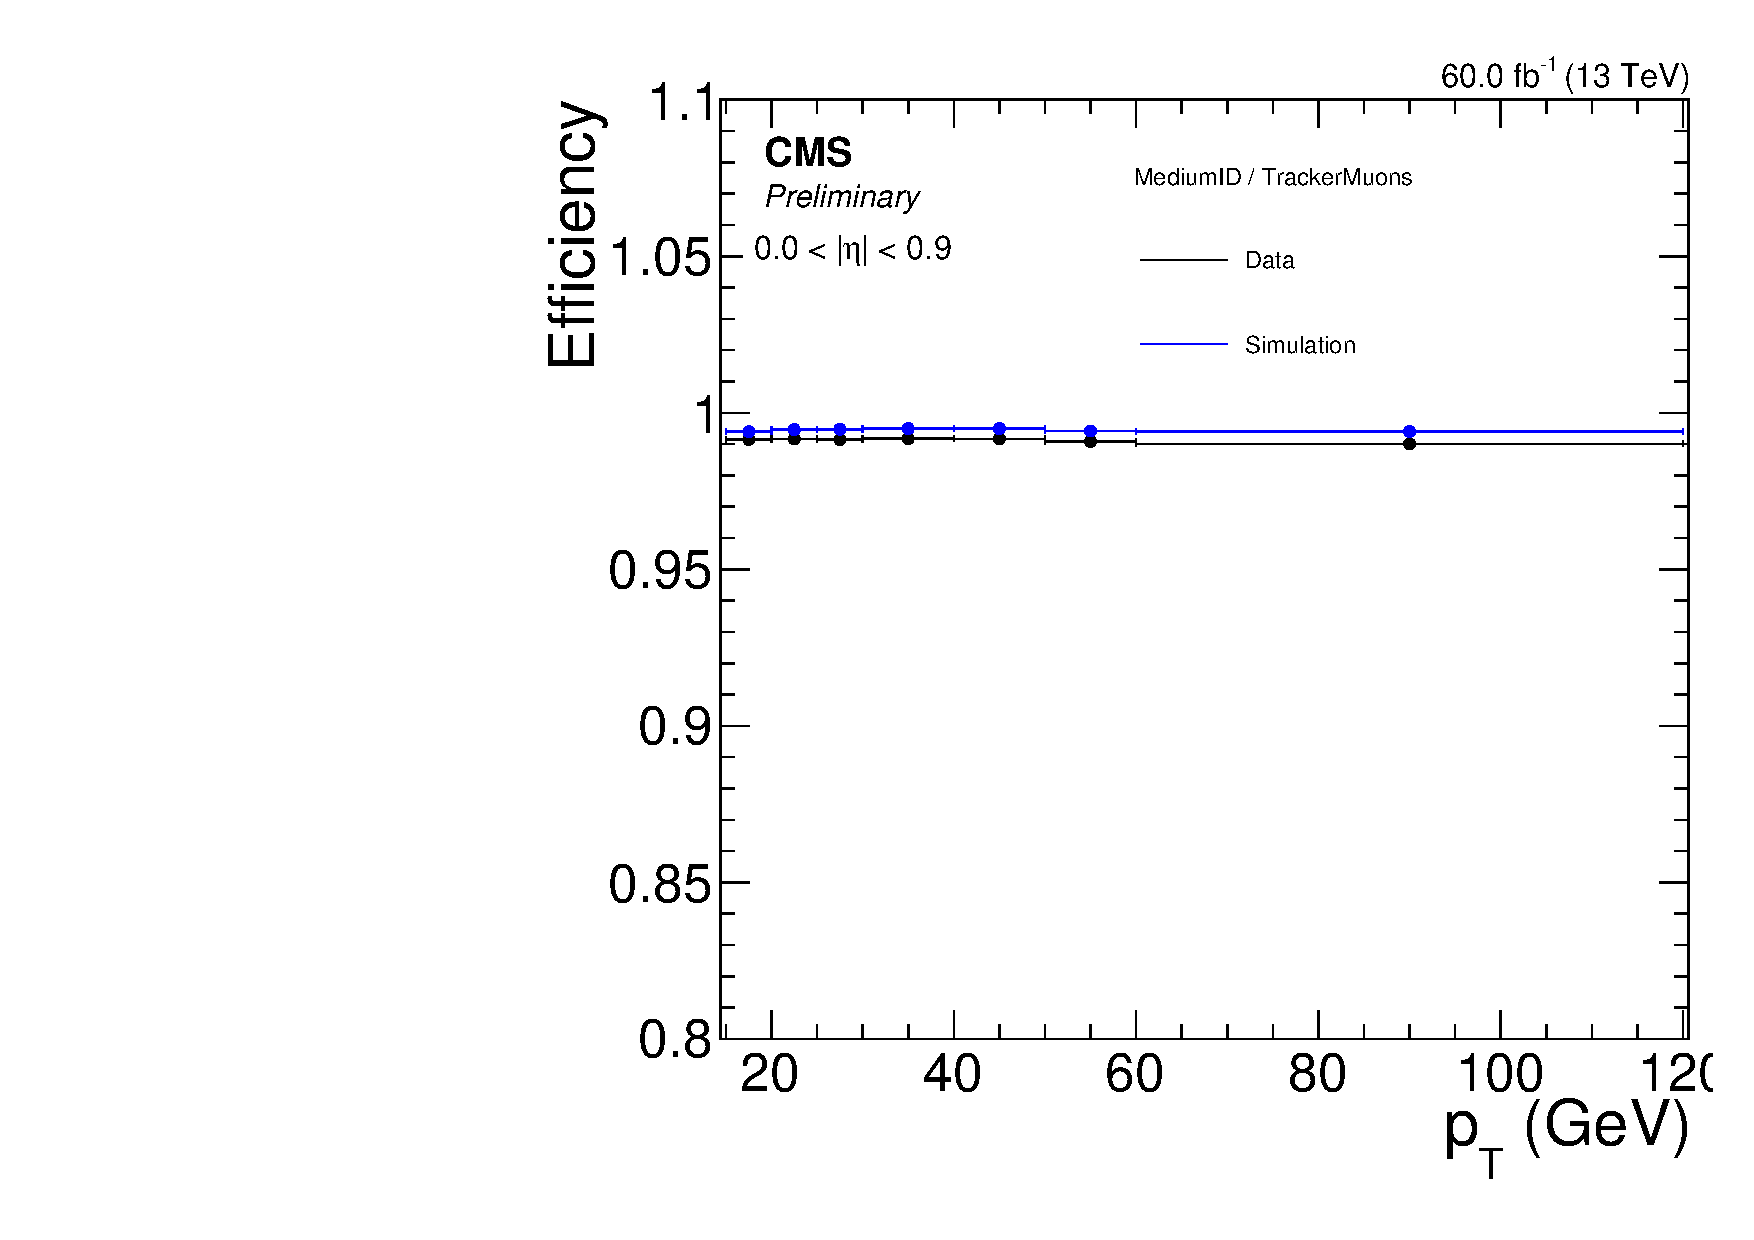
\includegraphics[width=0.49\textwidth]{Figures/Detector/CMS/muon_id_low_eta.pdf}
    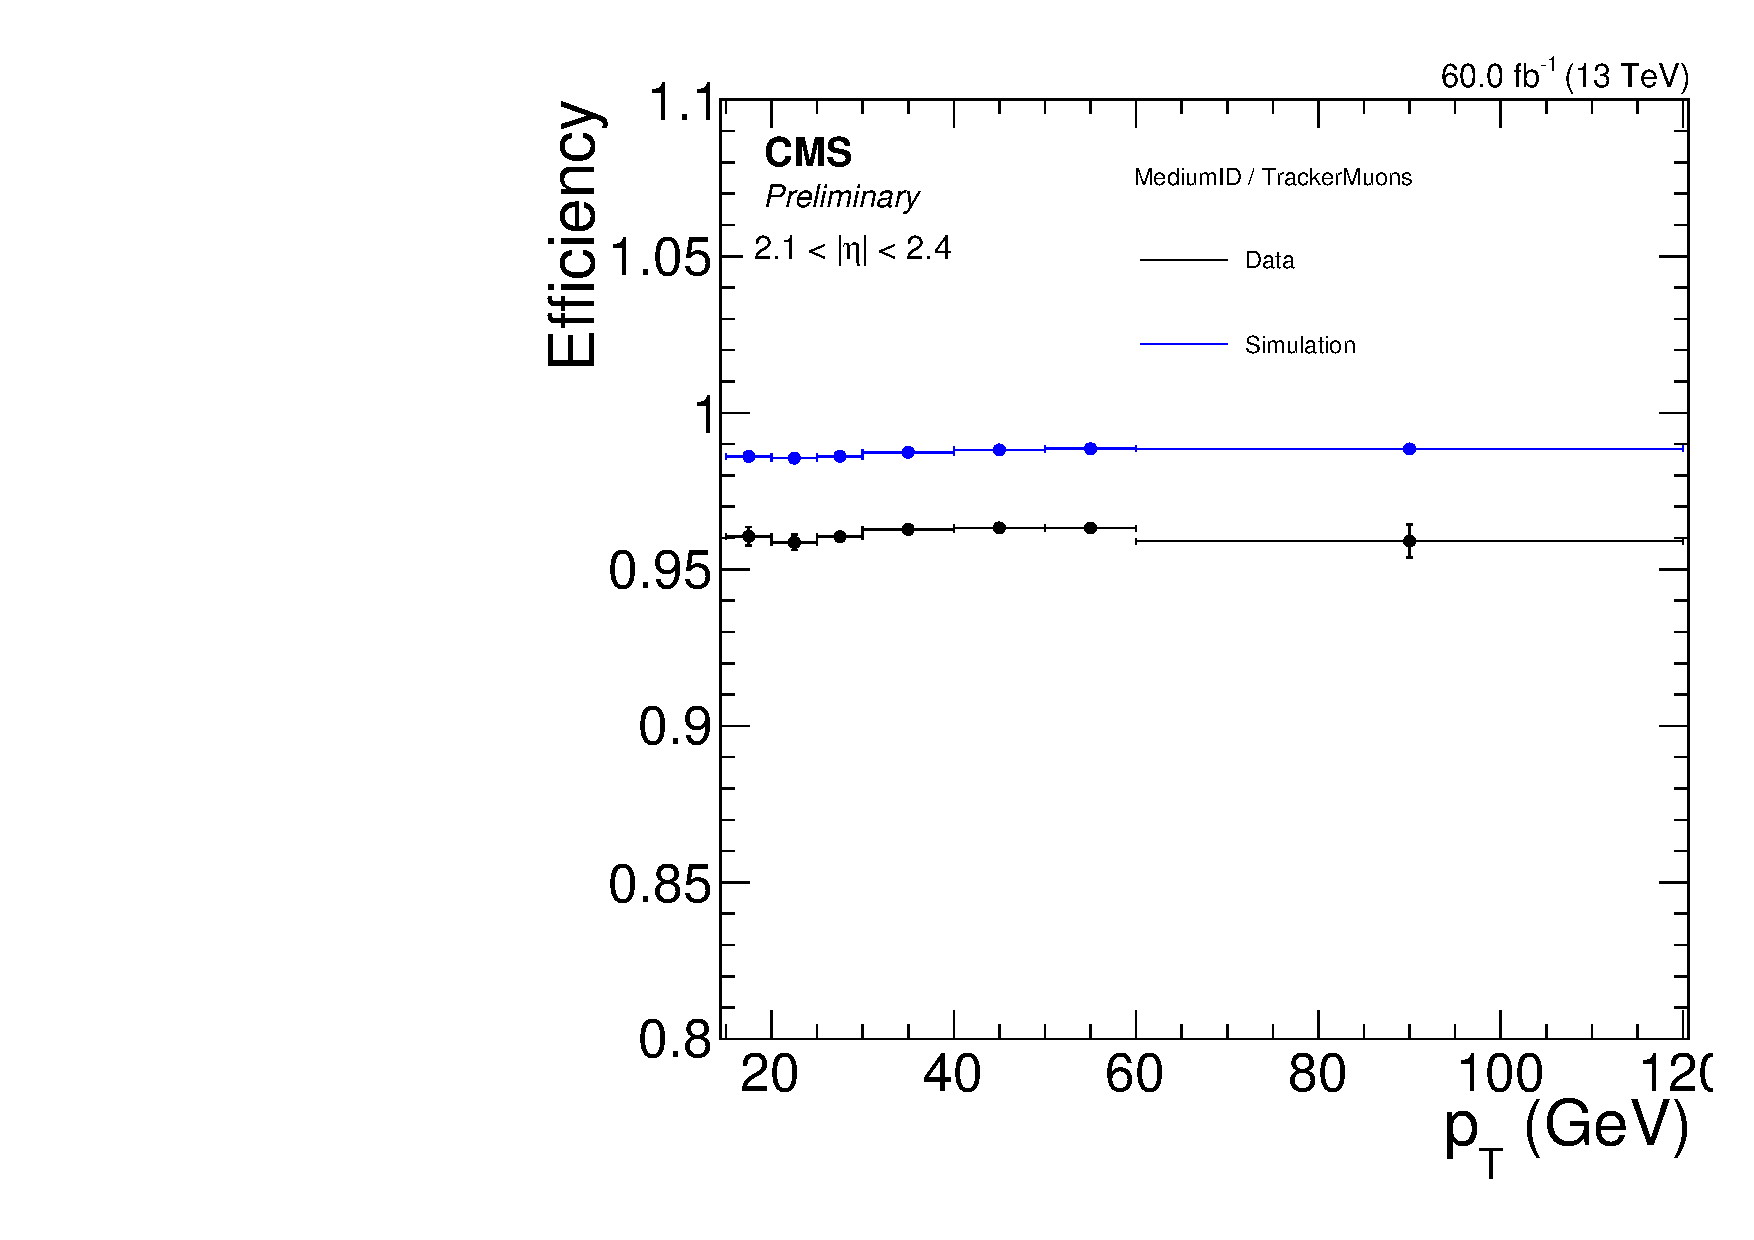
\includegraphics[width=0.49\textwidth]{Figures/Detector/CMS/muon_id_high_eta.pdf}
    \caption[Medium Muon ID Efficiency in 2018]{Medium muon ID efficiency in 2018 as measured in data and simulation as a function of muon \pt for $\abs{\eta} < 0.9$ (left) and $2.1 < \abs{\eta} < 2.4$ (right).}\label{fig:muon_id_performance}
  \end{figure}

\subsubsection{Muon Momentum}

Muon momentum is determined by the Tune-P algorithm~\cite{CMS:2012nsv} which selects the \pt measurement from different refits of the muon track based on the goodness-of-fit information and estimated \pt resolution. The types of refits include tracker-only, tracker and first muon detector plane, global without muon chambers with high occupancies, and a \textit{dynamic-truncation} fit which propagates the track to the muon stations but stops as soon as no compatible hit is found in two consecutive stations.

The momentum scale calibration and resolution estimation are derived from $\PZ/\gamma^*\to\mu\mu$, $J/\psi\to\mu\mu$ and $\Upsilon(1S)\to\mu\mu$ events in data~\cite{Bodek:2012id}. The momentum scale corrections are about 0.2\% and 0.3\% in the barrel and endcap respectively, and the resolution is about 1\% in the barrel and 3\% in the endcap for muons with \pt up to 100\GeV. The momentum resolution of intermediate and high \pt muons is additionally measured in cosmic ray events by comparing the momentum measurements in the upper and lower halves of the detector~\cite{CMS:2009fdy}. The momentum resolution, as measured with this method in 2015 data, is shown in \cref{fig:muon_resolution}. 

\begin{figure}
  \centering
  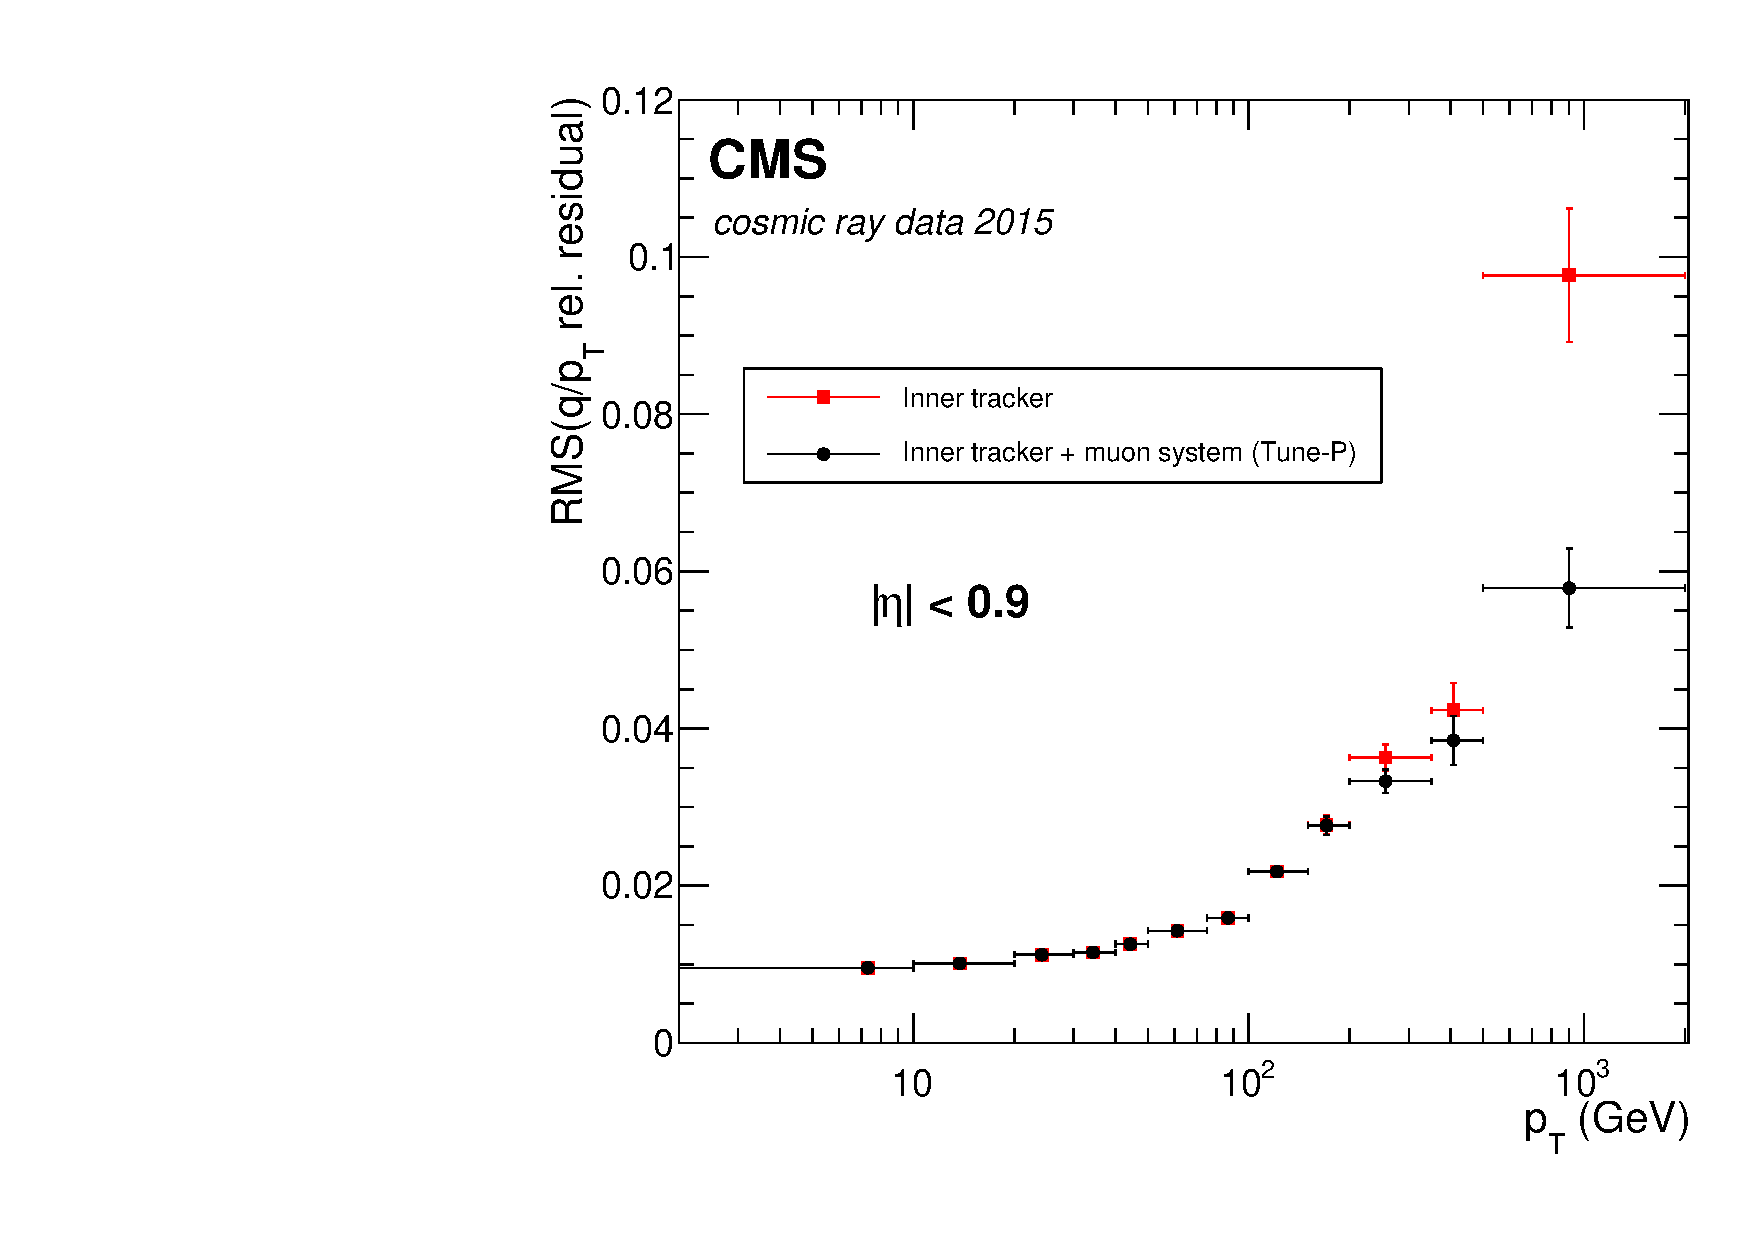
\includegraphics[width=0.7\textwidth]{Figures/Detector/CMS/muon_momentum_resolution.pdf}
  \caption[Muon Momentum Resolution as a Function of \pt]{Relative muon momentum resolution as a function of \pt for $\abs{\eta} < 0.9$ measured using cosmic ray data collected in 2015. The vertical error bars indicate statistical uncertainties. Figure taken from Ref.~\cite{CMS:2018rym}.}\label{fig:muon_resolution}
\end{figure}